%%%%%%%%%%%%%%%%%%%%%%%%%%%%%%%%%%%%%%%%%
% Short Sectioned Assignment
% LaTeX Template
% Version 1.0 (5/5/12)
%
% This template has been downloaded from:
% http://www.LaTeXTemplates.com
%
% Original author:
% Frits Wenneker (http://www.howtotex.com)
%
% License:
% CC BY-NC-SA 3.0 (http://creativecommons.org/licenses/by-nc-sa/3.0/)
%
%%%%%%%%%%%%%%%%%%%%%%%%%%%%%%%%%%%%%%%%%

%----------------------------------------------------------------------------------------
% PACKAGES AND OTHER DOCUMENT CONFIGURATIONS
%----------------------------------------------------------------------------------------

\documentclass[paper=a4, fontsize=11pt]{scrartcl} % A4 paper and 11pt font size

\usepackage[T1]{fontenc} % Use 8-bit encoding that has 256 glyphs
\usepackage{fourier} % Use the Adobe Utopia font for the document - comment this line to return to the LaTeX default
\usepackage[english]{babel} 
\usepackage[utf8]{inputenc}
\usepackage{amsmath,amsfonts,amsthm} % Math packages
\usepackage{tikz} % drawing package

\usepackage{sectsty} % Allows customizing section commands
\allsectionsfont{\centering \normalfont\scshape} % Make all sections centered, the default font and small caps

\usepackage{fancyhdr} % Custom headers and footers
\pagestyle{fancyplain} % Makes all pages in the document conform to the custom headers and footers
\fancyhead{} % No page header - if you want one, create it in the same way as the footers below
\fancyfoot[L]{} % Empty left footer
\fancyfoot[C]{} % Empty center footer
\fancyfoot[R]{\thepage} % Page numbering for right footer
\renewcommand{\headrulewidth}{0pt} % Remove header underlines
\renewcommand{\footrulewidth}{0pt} % Remove footer underlines
\setlength{\headheight}{13.6pt} % Customize the height of the header

\numberwithin{equation}{section} % Number equations within sections (i.e. 1.1, 1.2, 2.1, 2.2 instead of 1, 2, 3, 4)
\numberwithin{figure}{section} % Number figures within sections (i.e. 1.1, 1.2, 2.1, 2.2 instead of 1, 2, 3, 4)
\numberwithin{table}{section} % Number tables within sections (i.e. 1.1, 1.2, 2.1, 2.2 instead of 1, 2, 3, 4)

\setlength\parindent{0pt} % Removes all indentation from paragraphs - comment this line for an assignment with lots of text

%---- Listings --------------
\usepackage{color}
\definecolor{light-gray}{gray}{0.95}
\usepackage{listings}

\lstset{ %
language=C,                % choose the language of the code
basicstyle=\footnotesize,       % the size of the fonts that are used for the code
numbers=left,                   % where to put the line-numbers
numberstyle=\footnotesize,      % the size of the fonts that are used for the line-numbers
stepnumber=1,                   % the step between two line-numbers. If it is 1 each line will be numbered
resetmargins=true,              % reset line numbers
numbersep=5pt,                  % how far the line-numbers are from the code
backgroundcolor=\color{white},  % choose the background color. You must add \usepackage{color}
showspaces=false,               % show spaces adding particular underscores
showstringspaces=false,         % underline spaces within strings
showtabs=false,                 % show tabs within strings adding particular underscores
frame=single,           % adds a frame around the code
tabsize=2,          % sets default tabsize to 2 spaces
captionpos=b,           % sets the caption-position to bottom
breaklines=true,        % sets automatic line breaking
breakatwhitespace=false,    % sets if automatic breaks should only happen at whitespace
escapeinside={\%*}{*)}          % if you want to add a comment within your code
}

%----------------------------------------------------------------------------------------
% TITLE SECTION
%----------------------------------------------------------------------------------------

\newcommand{\horrule}[1]{\rule{\linewidth}{#1}} % Create horizontal rule command with 1 argument of height

\title{ 
\normalfont \normalsize 
\textsc{TDT4205 Compilers, NTNU} \\ [25pt] % Your university, school and/or department name(s)
\horrule{0.5pt} \\[0.4cm] % Thin top horizontal rule
\huge Problem Set 4 \\ % The assignment title
\horrule{2pt} \\[0.5cm] % Thick bottom horizontal rule
}

\author{Stian Jensen} % Your name

\date{\normalsize 24. februar 2014} % Today's date or a custom date

\begin{document}

\maketitle % Print the title

%----------------------------------------------------------------------------------------
% PROBLEM 1
%----------------------------------------------------------------------------------------

\section{Symbol tables}

%----------------------------------------------------------------------------------------
\subsection{Part a)}

A symbol table keeps track of identifiers used in a source program.



%----------------------------------------------------------------------------------------
\subsection{Part b)}

A symbol table typically stores the identifiers occurence in the program, along with other related information, such as type and scope level.

%----------------------------------------------------------------------------------------
\subsection{Part c)}

For implementing a symbol table one could use either a hash table, a list, or a binary heap.
We'd want to use the data structure that gives the best efficiency for our symbol table.
A list can provide O(1) for insertions, but retrieval is O(n).
A binary heap has O(n log n) for both insertions and retrievals.
A hash table, however, can both insert and lookup in near constant time.
A hash table would therefore be the best choice for a symbol table.

%----------------------------------------------------------------------------------------
% PROBLEM 2
%----------------------------------------------------------------------------------------

\newpage
\section{Symbol tables and blocks}

\subsection{Part a)}

Position 1

\begin{table}[ht!]
    \center
    \begin{tabular}{|l|l|}
    \hline
    Symbol name & Type           \\ \hline
    b        & bool \\ \hline
    \end{tabular}
    \caption{Top level}
\end{table}

\begin{table}[ht!]
    \begin{center}
    \begin{tabular}{|l|l|}
    \hline
    Symbol name & Type           \\ \hline
    a        & int   \\ \hline
    b        & float \\ \hline
    \end{tabular}
    \end{center}
\end{table}

\begin{table}[ht!]
    \center
    \begin{tabular}{|l|l|}
    \hline
    Symbol name & Type           \\ \hline
    main        & function, void \\ \hline
    \end{tabular}
\end{table}

Position 2

\begin{table}[ht!]
    \center
    \begin{tabular}{|l|l|}
    \hline
    Symbol name & Type           \\ \hline
    a        & bool \\ \hline
    c        & int \\ \hline
    \end{tabular}
\end{table}

\begin{table}[ht!]
    \center
    \begin{tabular}{|l|l|}
    \hline
    Symbol name & Type           \\ \hline
    b        & int \\ \hline
    c        & float \\ \hline
    \end{tabular}
\end{table}

\begin{table}[ht!]
    \center
    \begin{tabular}{|l|l|}
    \hline
    Symbol name & Type           \\ \hline
    a        & int   \\ \hline
    b        & float \\ \hline
    \end{tabular}
\end{table}

\begin{table}[ht!]
    \center
    \begin{tabular}{|l|l|}
    \hline
    Symbol name & Type           \\ \hline
    main        & function, void \\ \hline
    \end{tabular}
\end{table}

\subsection{Part b)}

\subsubsection{Position 1:}
\begin{table}[ht!]
    \center
    \begin{tabular}{|l|l|l|}
    \hline
    Symbol name & Type           & Scope depth \\ \hline
    main        & function, void & 0 \\ \hline
    a        & int     & 1 \\ \hline
    b        & float   & 1 \\ \hline
    b        & bool    & 2 \\ \hline
    \end{tabular}
\end{table}

\subsubsection{Position 2:}
\begin{table}[ht!]
    \center
    \begin{tabular}{|l|l|l|}
    \hline
    Symbol name & Type           & Scope depth \\ \hline
    main        & function, void & 0 \\ \hline
    a        & int     & 1 \\ \hline
    b        & float   & 1 \\ \hline
    b        & int    & 2 \\ \hline
    c        & float  & 2 \\ \hline
    a        & bool   & 3 \\ \hline
    c        & int    & 3 \\ \hline
    \end{tabular}
\end{table}

\subsection{Part c)}

With a single hash table, the lookup time for a symbol will always be O(1).

With multiple symbol tables, however, it's easier to see which variables are defined in a particular scope. But it also means you may have to search through multiple hash tables to find the symbol you are looking for.

\section{Type checking}

\subsection{Part a)}
Type synthesizing means obtaining the type of something by looking at the types of its subparts.
For the example y = x + z, if x is an integer and z is a float, we know that y must be float.

Type inference means finding the type of something by looking at how it's used.

\subsection{Part b)}

I assume that a double is twice the size of a float, and that an int and a float are the same size.

\begin{table}[ht!]
    \center
    \begin{tabular}{|l|l|}
    \hline
    Data Type   & Widenes to data type \\ \hline
    Integer & Integer, Float, Double, Complex integer, Complex float, Complex double \\
    Float & Float, Double, Complex float, Complex double \\
    Double & Double, Complex double \\
    Complex integer & Complex integer, Complex float, Complex double \\
    Complex float & Complex float, Complex double \\
    Complex double & Complex double \\ \hline
    \end{tabular}
\end{table}

\section{Types, SDDs}

\subsection{Part a)}

\begin{table}[ht!]
    \center
    \begin{tabular}{|l|l|}
    \hline
    Production   & Semantic rule   \\ \hline
    T ::= int    & T.size = 4 \\
    T ::= float  & T.size = 8 \\
    T ::= bool   & T.size = 1 \\
    T ::= T[num] & T.size = T.size * num \\
    T ::= (L)    & T.size = L.size \\
    L ::= L,T    & L.size = L.size + T.size \\
    L ::= T      & L.size = T.size \\ \hline
    \end{tabular}
\end{table}

\newpage
\subsection{Part b)}

\subsubsection{i}

\begin{figure}[ht!]
\centering
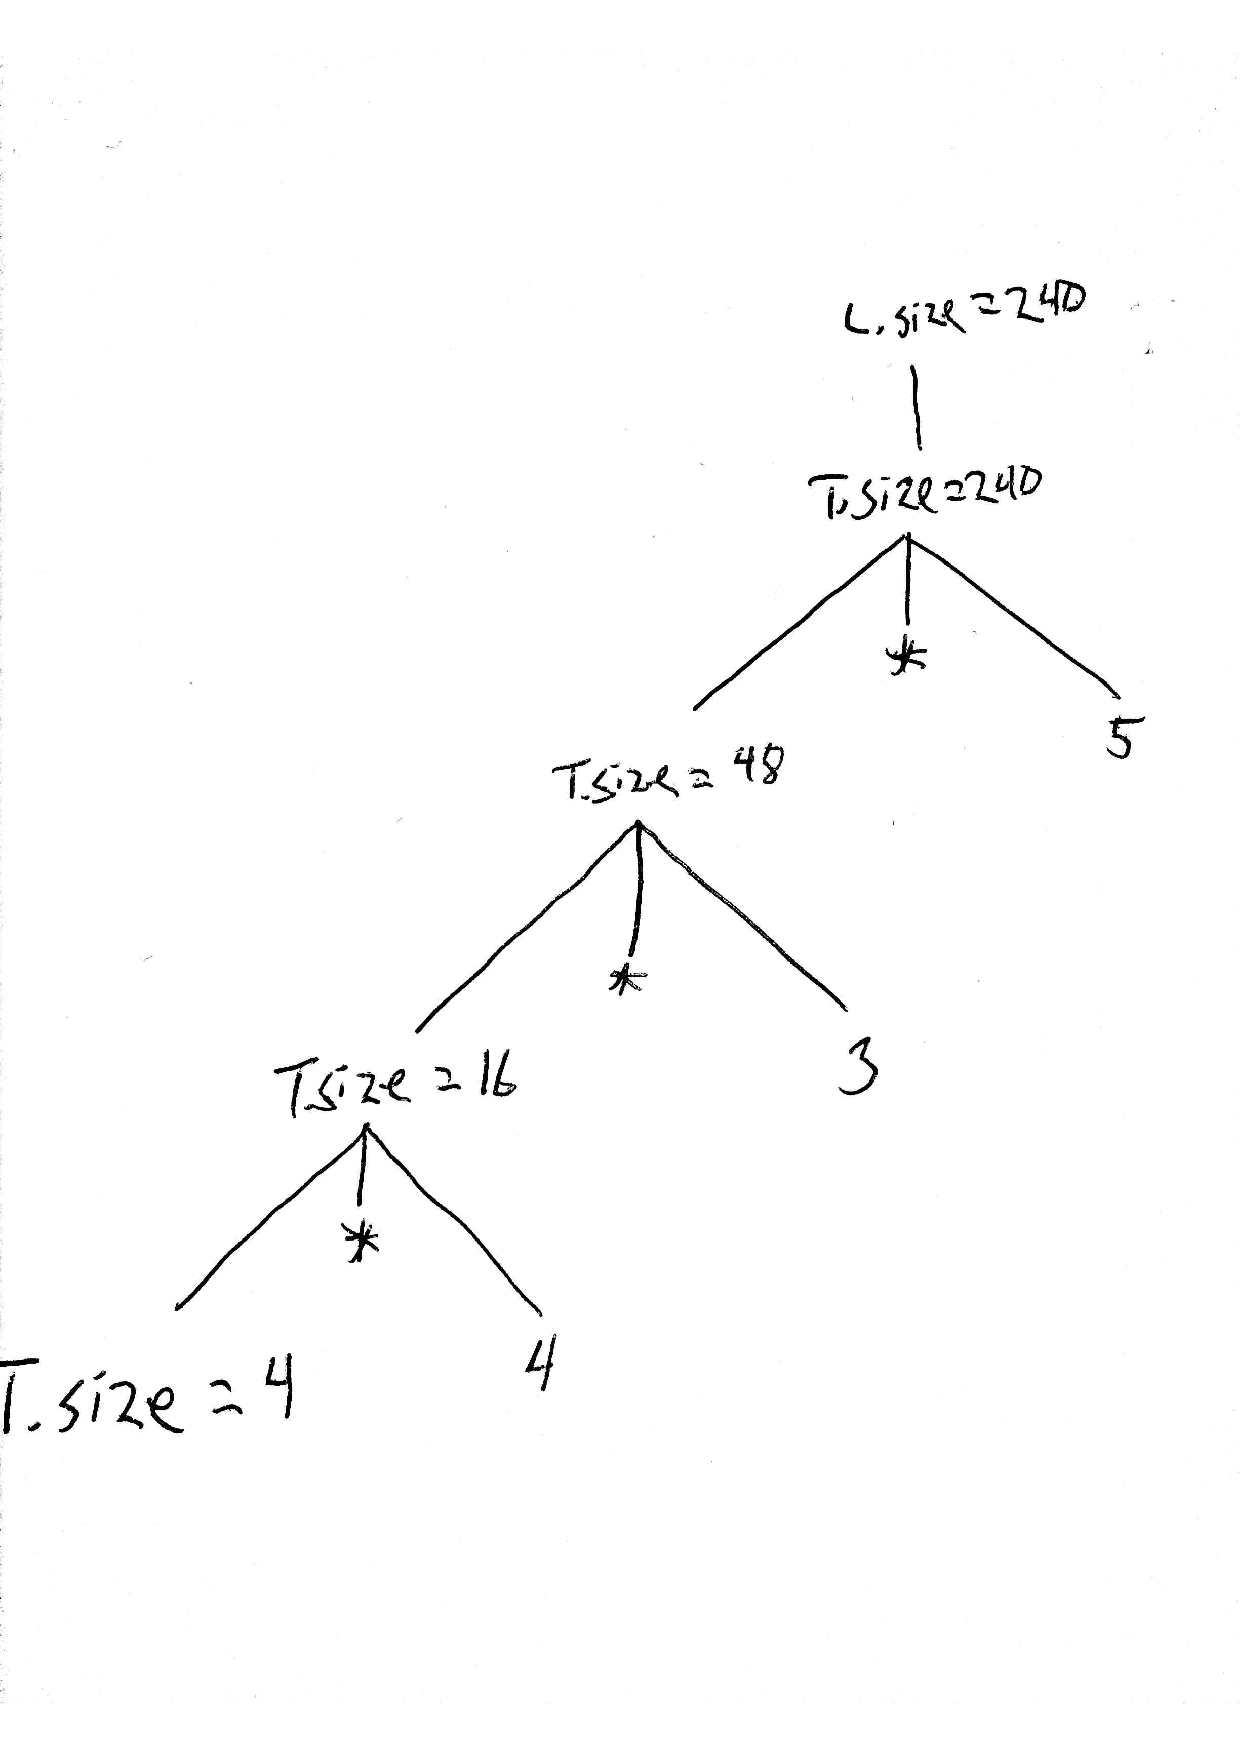
\includegraphics[width=90mm]{task_b_i.pdf}
\end{figure}

\newpage
\subsubsection{ii}
\begin{figure}[ht!]
\centering
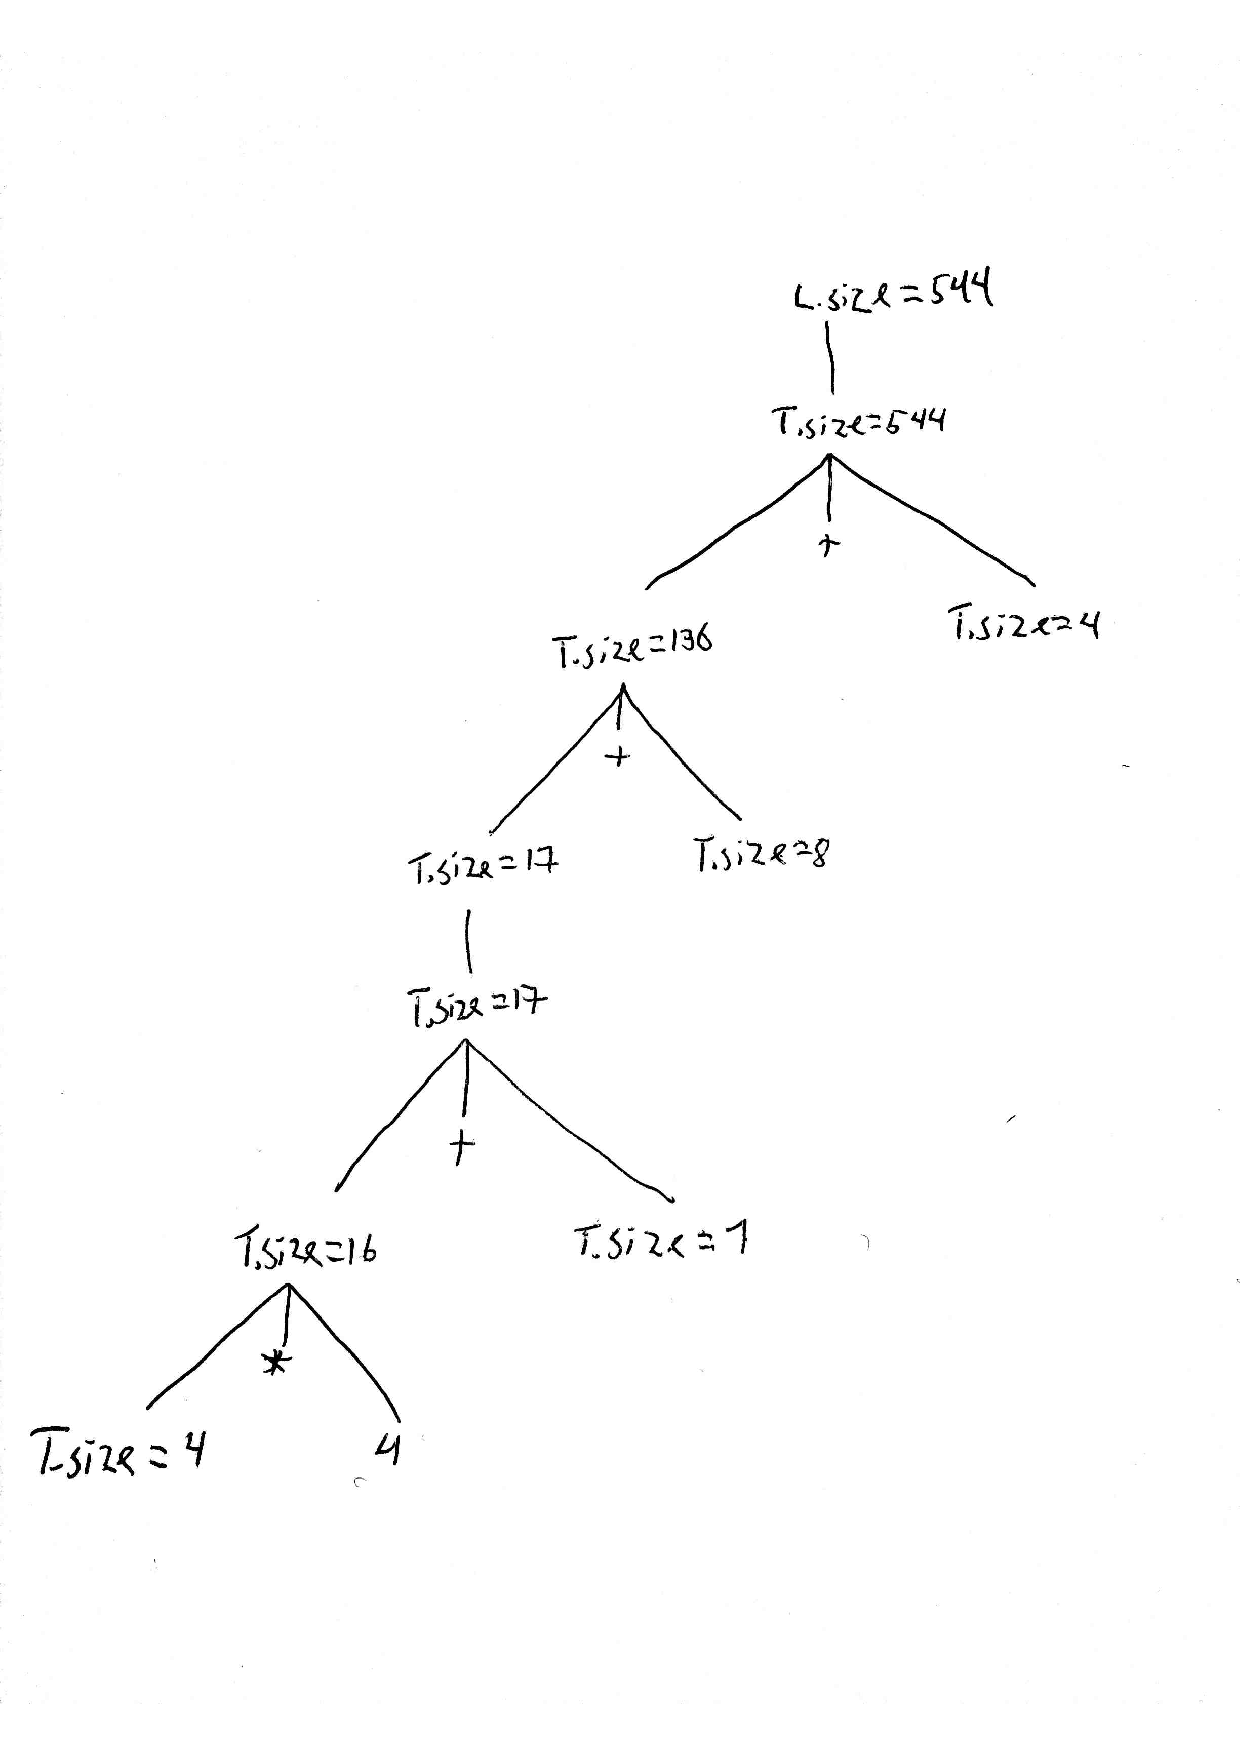
\includegraphics[width=90mm]{task_b_ii.pdf}
\end{figure}


%----------------------------------------------------------------------------------------

\end{document}
